%!TeX root=../sensetop.tex
\chapter[Chapter \thechapter]{}
\lettrine[lines=4,lraise=0.3]{I}{n} a firm, though cautious tone, Elinor thus began.

\zz
»I should be undeserving of the confidence you have honoured me with, if I felt no desire for its continuance, or no farther curiosity on its subject. I will not apologize therefore for bringing it forward again.«

»Thank you,« cried Lucy warmly, »for breaking the ice; you have set my heart at ease by it; for I was somehow or other afraid I had offended you by what I told you that Monday.«

»Offended me! How could you suppose so? Believe me,« and Elinor spoke it with the truest sincerity, »nothing could be farther from my intention than to give you such an idea. Could you have a motive for the trust, that was not honourable and flattering to me?«

»And yet I do assure you,« replied Lucy, her little sharp eyes full of meaning, »there seemed to me to be a coldness and displeasure in your manner that made me quite uncomfortable. I felt sure that you was angry with me; and have been quarrelling with myself ever since, for having took such a liberty as to trouble you with my affairs. But I am very glad to find it was only my own fancy, and that you really do not blame me. If you knew what a consolation it was to me to relieve my heart speaking to you of what I am always thinking of every moment of my life, your compassion would make you overlook every thing else I am sure.«

»Indeed, I can easily believe that it was a very great relief to you, to acknowledge your situation to me, and be assured that you shall never have reason to repent it. Your case is a very unfortunate one; you seem to me to be surrounded with difficulties, and you will have need of all your mutual affection to support you under them. Mr Ferrars, I believe, is entirely dependent on his mother.«

»He has only two thousand pounds of his own; it would be madness to marry upon that, though for my own part, I could give up every prospect of more without a sigh. I have been always used to a very small income, and could struggle with any poverty for him; but I love him too well to be the selfish means of robbing him, perhaps, of all that his mother might give him if he married to please her. We must wait, it may be for many years. With almost every other man in the world, it would be an alarming prospect; but Edward’s affection and constancy nothing can deprive me of I know.«

»That conviction must be every thing to you; and he is undoubtedly supported by the same trust in your’s. If the strength of your reciprocal attachment had failed, as between many people, and under many circumstances it naturally would during a four years’ engagement, your situation would have been pitiable, indeed.«

Lucy here looked up; but Elinor was careful in guarding her countenance from every expression that could give her words a suspicious tendency.

»Edward’s love for me,« said Lucy, »has been pretty well put to the test, by our long, very long absence since we were first engaged, and it has stood the trial so well, that I should be unpardonable to doubt it now. I can safely say that he has never gave me one moment’s alarm on that account from the first.«

Elinor hardly knew whether to smile or sigh at this assertion.

Lucy went on. »I am rather of a jealous temper too by nature, and from our different situations in life, from his being so much more in the world than me, and our continual separation, I was enough inclined for suspicion, to have found out the truth in an instant, if there had been the slightest alteration in his behaviour to me when we met, or any lowness of spirits that I could not account for, or if he had talked more of one lady than another, or seemed in any respect less happy at Longstaple than he used to be. I do not mean to say that I am particularly observant or quick-sighted in general, but in such a case I am sure I could not be deceived.«

»All this,« thought Elinor, »is very pretty; but it can impose upon neither of us.«

»But what,« said she after a short silence, »are your views? or have you none but that of waiting for Mrs Ferrars’s death, which is a melancholy and shocking extremity?—Is her son determined to submit to this, and to all the tediousness of the many years of suspense in which it may involve you, rather than run the risk of her displeasure for a while by owning the truth?«

»If we could be certain that it would be only for a while! But Mrs Ferrars is a very headstrong proud woman, and in her first fit of anger upon hearing it, would very likely secure every thing to Robert, and the idea of that, for Edward’s sake, frightens away all my inclination for hasty measures.«

»And for your own sake too, or you are carrying your disinterestedness beyond reason.«

Lucy looked at Elinor again, and was silent.

»Do you know Mr Robert Ferrars?« asked Elinor.

»Not at all—I never saw him; but I fancy he is very unlike his brother—silly and a great coxcomb.«

»A great coxcomb!« repeated Miss Steele, whose ear had caught those words by a sudden pause in Marianne’s music. »Oh, they are talking of their favourite beaux, I dare say.«

»No sister,« cried Lucy, »you are mistaken there, our favourite beaux are \textit{not} great coxcombs.«

»I can answer for it that Miss Dashwood’s is not,« said Mrs Jennings, laughing heartily; »for he is one of the modestest, prettiest behaved young men I ever saw; but as for Lucy, she is such a sly little creature, there is no finding out who \textit{she} likes.«

\begin{figure}[tbph]
\centering
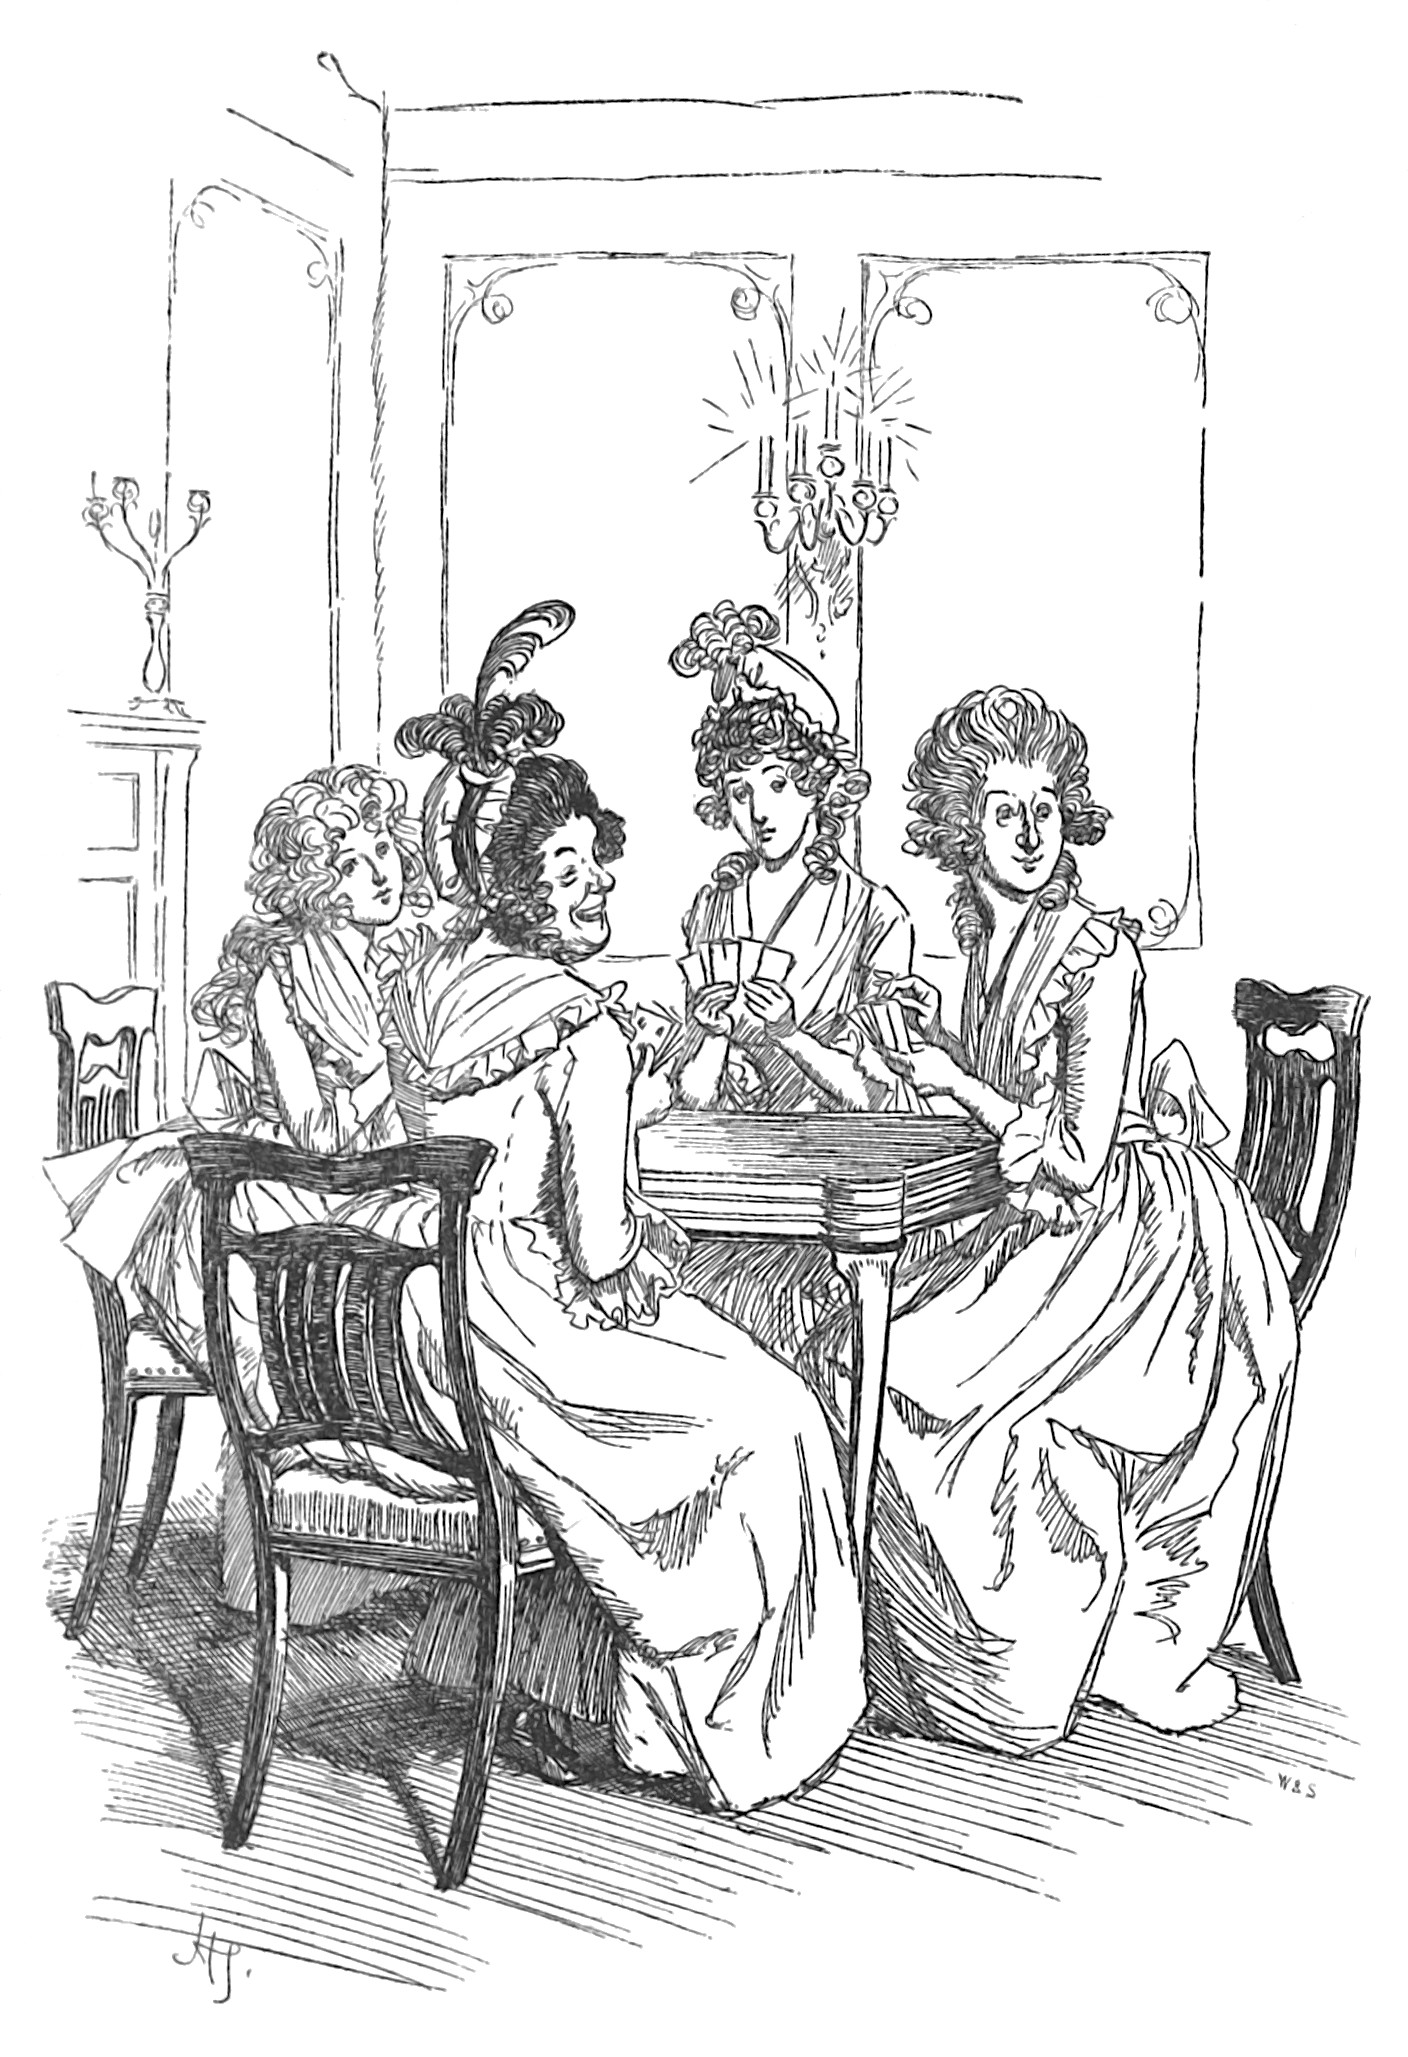
\includegraphics[width=\linewidth]{24answer}
\caption{»I can answer for it,« said Mrs Jennings}
\end{figure}

»Oh,« cried Miss Steele, looking significantly round at them, »I dare say Lucy’s beau is quite as modest and pretty behaved as Miss Dashwood’s.«

Elinor blushed in spite of herself. Lucy bit her lip, and looked angrily at her sister. A mutual silence took place for some time. Lucy first put an end to it by saying in a lower tone, though Marianne was then giving them the powerful protection of a very magnificent concerto,—

»I will honestly tell you of one scheme which has lately come into my head, for bringing matters to bear; indeed I am bound to let you into the secret, for you are a party concerned. I dare say you have seen enough of Edward to know that he would prefer the church to every other profession; now my plan is that he should take orders as soon as he can, and then through your interest, which I am sure you would be kind enough to use out of friendship for him, and I hope out of some regard to me, your brother might be persuaded to give him Norland living; which I understand is a very good one, and the present incumbent not likely to live a great while. That would be enough for us to marry upon, and we might trust to time and chance for the rest.«

»I should always be happy,« replied Elinor, »to show any mark of my esteem and friendship for Mr Ferrars; but do you not perceive that my interest on such an occasion would be perfectly unnecessary? He is brother to Mrs John Dashwood—\textit{that} must be recommendation enough to her husband.«

»But Mrs John Dashwood would not much approve of Edward’s going into orders.«

»Then I rather suspect that my interest would do very little.«

They were again silent for many minutes. At length Lucy exclaimed with a deep sigh,

»I believe it would be the wisest way to put an end to the business at once by dissolving the engagement. We seem so beset with difficulties on every side, that though it would make us miserable for a time, we should be happier perhaps in the end. But you will not give me your advice, Miss Dashwood?«

»No,« answered Elinor, with a smile, which concealed very agitated feelings, »on such a subject I certainly will not. You know very well that my opinion would have no weight with you, unless it were on the side of your wishes.«

»Indeed you wrong me,« replied Lucy, with great solemnity; »I know nobody of whose judgment I think so highly as I do of yours; and I do really believe, that if you was to say to me, »I advise you by all means to put an end to your engagement with Edward Ferrars, it will be more for the happiness of both of you,« I should resolve upon doing it immediately.«

Elinor blushed for the insincerity of Edward’s future wife, and replied, »This compliment would effectually frighten me from giving any opinion on the subject had I formed one. It raises my influence much too high; the power of dividing two people so tenderly attached is too much for an indifferent person.«

»’Tis because you are an indifferent person,« said Lucy, with some pique, and laying a particular stress on those words, »that your judgment might justly have such weight with me. If you could be supposed to be biased in any respect by your own feelings, your opinion would not be worth having.«

Elinor thought it wisest to make no answer to this, lest they might provoke each other to an unsuitable increase of ease and unreserve; and was even partly determined never to mention the subject again. Another pause therefore of many minutes’ duration, succeeded this speech, and Lucy was still the first to end it.

»Shall you be in town this winter, Miss Dashwood?« said she with all her accustomary complacency.

»Certainly not.«

»I am sorry for that,« returned the other, while her eyes brightened at the information, »it would have gave me such pleasure to meet you there! But I dare say you will go for all that. To be sure, your brother and sister will ask you to come to them.«

»It will not be in my power to accept their invitation if they do.«

»How unlucky that is! I had quite depended upon meeting you there. Anne and me are to go the latter end of January to some relations who have been wanting us to visit them these several years! But I only go for the sake of seeing Edward. He will be there in February, otherwise London would have no charms for me; I have not spirits for it.«

Elinor was soon called to the card-table by the conclusion of the first rubber, and the confidential discourse of the two ladies was therefore at an end, to which both of them submitted without any reluctance, for nothing had been said on either side to make them dislike each other less than they had done before; and Elinor sat down to the card table with the melancholy persuasion that Edward was not only without affection for the person who was to be his wife; but that he had not even the chance of being tolerably happy in marriage, which sincere affection on \textit{her} side would have given, for self-interest alone could induce a woman to keep a man to an engagement, of which she seemed so thoroughly aware that he was weary.

From this time the subject was never revived by Elinor, and when entered on by Lucy, who seldom missed an opportunity of introducing it, and was particularly careful to inform her confidante, of her happiness whenever she received a letter from Edward, it was treated by the former with calmness and caution, and dismissed as soon as civility would allow; for she felt such conversations to be an indulgence which Lucy did not deserve, and which were dangerous to herself.

The visit of the Miss Steeles at Barton Park was lengthened far beyond what the first invitation implied. Their favour increased; they could not be spared; Sir John would not hear of their going; and in spite of their numerous and long arranged engagements in Exeter, in spite of the absolute necessity of returning to fulfil them immediately, which was in full force at the end of every week, they were prevailed on to stay nearly two months at the park, and to assist in the due celebration of that festival which requires a more than ordinary share of private balls and large dinners to proclaim its importance.